\documentclass[10pt, landscape]{article}
\usepackage[scaled=0.92]{helvet}
\usepackage{calc}
\usepackage{multicol}
\usepackage{ifthen}
\usepackage[a4paper,margin=3mm,landscape]{geometry}
\usepackage{amsmath,amsthm,amsfonts,amssymb}
\usepackage{color,graphicx,overpic}
\usepackage{hyperref}
\usepackage{newtxtext} 
\usepackage{enumitem}
\usepackage{amssymb}
\usepackage[table]{xcolor}
\usepackage{vwcol}
\usepackage{tikz}
% for relations
\usepackage{cancel}
\usepackage{ mathrsfs }
\setlist{nosep}

\pdfinfo{
  /Title (CS1231S.pdf)
  /Creator (TeX)
  /Producer (pdfTeX 1.40.0)
  /Author (Seamus)
  /Subject (Example)
  /Keywords (pdflatex, latex,pdftex,tex)}

% Turn off header and footer
\pagestyle{empty}

% redefine section commands to use less space
\makeatletter
\renewcommand{\section}{\@startsection{section}{1}{0mm}%
                                {-1ex plus -.5ex minus -.2ex}%
                                {0.5ex plus .2ex}%x
                                {\normalfont\large\bfseries}}
\renewcommand{\subsection}{\@startsection{subsection}{2}{0mm}%
                                {-1explus -.5ex minus -.2ex}%
                                {0.5ex plus .2ex}%
                                {\normalfont\normalsize\bfseries}}
\renewcommand{\subsubsection}{\@startsection{subsubsection}{3}{0mm}%
                                {-1ex plus -.5ex minus -.2ex}%
                                {1ex plus .2ex}%
                                {\normalfont\small\bfseries}}%
\renewcommand{\familydefault}{\sfdefault}
\renewcommand\rmdefault{\sfdefault}
% makes nested numbering (e.g. 1.1.1, 1.1.2, etc)
\renewcommand{\labelenumii}{\theenumii}
\renewcommand{\theenumii}{\theenumi.\arabic{enumii}.}
\renewcommand\labelitemii{•}
%  for logical not operator
\renewcommand{\lnot}{\mathord{\sim}}
\renewcommand{\bf}[1]{\textbf{#1}}
\newcommand{\abs}[1]{\vert #1 \vert}
\newcommand{\Mod}[1]{\ \mathrm{mod}\ #1}

\makeatother
\definecolor{myblue}{cmyk}{1,.72,0,.38}
\everymath\expandafter{\the\everymath \color{myblue}}
% Define BibTeX command
\def\BibTeX{{\rm B\kern-.05em{\sc i\kern-.025em b}\kern-.08em
    T\kern-.1667em\lower.7ex\hbox{E}\kern-.125emX}}
\let\iff\leftrightarrow
\let\Iff\Leftrightarrow
\let\then\rightarrow
\let\Then\Rightarrow

% Don't print section numbers
\setcounter{secnumdepth}{0}

\setlength{\parindent}{0pt}
\setlength{\parskip}{0pt plus 0.5ex}
%% this changes all items (enumerate and itemize)
\setlength{\leftmargini}{0.5cm}
\setlength{\leftmarginii}{0.5cm}
\setlist[itemize,1]{leftmargin=2mm,labelindent=1mm,labelsep=1mm}
\setlist[itemize,2]{leftmargin=4mm,labelindent=1mm,labelsep=1mm}

%My Environments
\newtheorem{example}[section]{Example}
% -----------------------------------------------------------------------

\begin{document}
\raggedright
\footnotesize
\begin{multicols}{4
    '}


% multicol parameters
% These lengths are set only within the two main columns
\setlength{\columnseprule}{0.25pt}
\setlength{\premulticols}{1pt}
\setlength{\postmulticols}{1pt}
\setlength{\multicolsep}{1pt}
\setlength{\columnsep}{2pt}

\begin{center}
    %
     \Large{\textbf{CS1231S}} \\
     \fbox{\small{AY20/21 Sem 1}}
    %  
\end{center}

\section{01. PROOFS}
\subsection{sets of numbers}
    $\mathbb{N}$ : natural numbers ($\mathbb{Z}_{\geq 0}$)
\\* $\mathbb{Z}$ : integers
\\* $\mathbb{Q}$ : rational numbers
\\* $\mathbb{R}$ : real numbers
\\* $\mathbb{C}$ : complex numbers

\subsection{basic properties of integers}
\begin{center}
    closure (under addition and multiplication)
    \\* $x+y \in \mathbb{Z} \land xy \in \mathbb{Z}$

    commutativity
    \\* $a + b = b + a \land ab = ba$

    associativity
    \\* $a + b + c = a + (b + c) = (a + b) + c$
    \\* $abc = a(bc) = (ab)c$

    distributivity
    \\* $a(b + c) = ab + ac$

    trichotomy
    \\* $(a < b) \lor (a > b) \lor (a = b)$

    transitive law
    \\* $(a < b) \land (b < c) \implies (a < c)$
\end{center}
 
\subsection{definitions}
\begin{center}
    even/odd
    \\* $n \text{ is even} \iff \exists k \in \mathbb{Z} \mid n = 2k$
    \\* $n \text{ is odd} \iff \exists k \in \mathbb{Z} \mid n = 2k + 1$

    prime/composite
    \\* $n \text{ is prime} \iff n>1 \text{ and } \forall r, s \in \mathbb{Z}^+, n=rs \then (r=n)\lor(r=s)$
    \\* $n \text{ is composite} \iff n>1 \text{ and } \exists r, s \in \mathbb{Z}^+ s.t. n = rs \text{ and } 1<r<n \text{ and } 1<s<n$

    divisibility ($d$ divides $n$)
    \\* $d \mid n \iff \exists k \in \mathbb{Z} \mid n = kd$

    rationality
    \\* $r \text{ is rational} \iff \exists a, b \in \mathbb{Z} \mid r = \frac{a}{b} \text{ and } b \neq 0$

    floor/ceiling
    \\* $\lfloor x \rfloor$ : largest integer $y$ such that $y \leq x$
    \\* $\lceil x \rceil$ : smallest integer $y$ such that $y \geq x$
\subsubsection{rules of inference}
    \begin{multicols}{2}
        generalisation
        \\* $p,\ \therefore p \lor q$
        
        specialisation
        \\* $p \land q,\ \therefore p$

        elimination
        \\* $p \lor q;\ \ \lnot q,\ \therefore p$

        transitivity
        \\* $p \then q;\ q \then r;\ \ \therefore p \then r$
    \end{multicols}
\end{center}

\section{04. METHODS OF PROOF}
\subsection{Proof by Exhaustion/Cases}
\begin{enumerate}
    \item list out possible cases
    \begin{enumerate}
        \item Case 1: $n$ is odd OR If $n = 9$, ...
        \item Case 2: $n$ is even OR If $n = 16$, ...
    \end{enumerate}
    \item therefore ...
\end{enumerate}

\subsection{Proof by Contradiction}
\begin{enumerate}
    \item Suppose that \dots
    \begin{enumerate}
        \item <proof>
        \item \dots but this contradicts \dots
    \end{enumerate}
    \item Therefore the assumption that \dots is false. \\* Hence \dots.
\end{enumerate}

\subsection{Proof by Contraposition}
\begin{enumerate}
    \item Contrapositive statement: $\lnot q \then \lnot p$
    \item let $\lnot q$
    \begin{enumerate}
        \item <proof>
        \item hence $\lnot p$
    \end{enumerate}
    \item $\therefore p \then q$
\end{enumerate}

\subsection{Proof by Construction}
\begin{enumerate}
    \item Let $x = 3, y=4, z=5$.
    \item Then $x, y, z \in \mathbb{Z}_{\geq 1}$ and $x^2 + y^2 = 3^2 + 4^2 = 9 + 16 = 25 = 5^2$.
    \item Thus $\exists x, y, z \in \mathbb{Z}_{\geq 1}$ such that $x^2 + y^2 = z^2$.
\end{enumerate}

\subsection{Proof by Induction}
\begin{enumerate}
    \item For each $n \in \mathbb{Z}_{\geq 1}$, let $P(n)$ be the proposition "$\dots$"
    \item (base step) $P(1)$ is true because <manual method>
    \item (induction step) 
    \begin{enumerate}
        \item let $k \in \mathbb{Z}_{\geq 1}$ s.t. $P(k)$ is true
        \item Then \dots
        \item proof that $P(k + 1)$ is true - e.g. $P(k+1) = P(k) + term_{k+1}$
        \item So $P(k + 1)$ is true.
    \end{enumerate}
    \item Hence $\forall n \in \mathbb{Z}_{\geq 1} P(n)$ is true by MI.
\end{enumerate}

\subsection{Proofs for Sets}
\bf{Equality of Sets (A=B)}
\begin{enumerate}
    \item $(\Rightarrow)$
        \begin{enumerate}
            \item Take any $z \in A$.
            \item $\dots$
            \item $\therefore z \in B$.
        \end{enumerate}
    \item $(\Leftarrow)$
    \begin{enumerate}
        \item Take any $z \in B$.
        \item $\dots$
        \item $\therefore z \in A$.
    \end{enumerate}
\end{enumerate}

\bf{Element Method}
\begin{enumerate}
    \item $A \cap (B \backslash C) = \{ x : x \in A \land x \in (B \backslash C) \}$ (by def. of $\cap$)
    \item $= \{ x : x \in A \land (x \in B \land x \notin C)\}$ (by def. of $\backslash$)
    \item $\dots$
    \item $= (A \cap B) \backslash C$ (by def. of $\backslash$)
\end{enumerate}

\subsection{Other Proofs}
\bf{iff ($A \iff B$)}
\begin{enumerate}
    \item ($\Rightarrow$) Suppose $A$.
    \begin{enumerate}
        \item $\dots$ <proof> $\dots$
        \item Hence $A \then B$
    \end{enumerate}
    \item ($\Leftarrow$) Suppose $B$.
    \begin{enumerate}
        \item $\dots$ <proof> $\dots$
        \item Hence $B \then A$
    \end{enumerate}
\end{enumerate}

\section{02. COMPOUND STATEMENTS}
\subsection{operations}
\begin{itemize}
    \item[1] $\sim$ : negation (not)
    \item[2] $\land$ : conjunction (and)
    \item[2] $\lor$ : disjunction (or) - coequal to $\land$
    \item[3] $\rightarrow$ : if-then
\end{itemize}

\subsubsection{logical equivalence} 
\begin{itemize}
    \item identical truth values in truth table
    \item definitions
    \item to show non-equivalence: 
    \begin{itemize}
        \item truth table method (only needs 1 row)
        \item counter-example method
    \end{itemize}
\end{itemize}

\subsection{conditional statements}
    \begin{equation*}
        \begin{split}
            \text{hypothesis} &\then \text{conclusion} \\
            antecedent &\then consequent
        \end{split}
    \end{equation*}

\begin{itemize}
    \item \textbf{vacuously true} : hypothesis is false
    \item \textbf{implication law} : $p \then q \equiv \lnot p \lor q$
    \item common if/then statements:
    \begin{itemize}
        \item if p then q: $p \then q$
        \item p if q: $q \then p$
        \item p only if q: $p \then q$
        \item p iff q: $p \iff q$
    \end{itemize}
\end{itemize}

\setlength{\tabcolsep}{0.3em}
\begin{tabular}{>{\color{black}}p{0.12\textwidth}| >{\color{black}}p{0.08\textwidth}}
    \begin{itemize}
        \item \bf{contrapositive} : $\lnot q \then \lnot p$ 
        \item \bf{inverse} : $\lnot p \then \lnot q$ 
        \item \bf{converse} : $q \then p$ 
    \end{itemize} 
    & converse $\equiv$ inverse \newline
    statement $\equiv$ contrapositive
\end{tabular}
\begin{itemize}
    \item r is a \bf{necessary} condition for s: $\lnot r \then \lnot s$ and $s \then r$
    \item r is a \bf{sufficient} condition for s: $r \then s$
    \item \bf{necessary} \& \bf{sufficient} : $\iff$
\end{itemize}

\subsection{valid arguments}
\begin{itemize}
    \item determining validity: construct truth table
    \begin{itemize}
        \item valid $\iff$ conclusion is true when premises are true
    \end{itemize}
    \item \bf{syllogism} : (argument form) 2 premises, 1 conclusion
    \item \bf{modus ponens} : $p \then q;\ p;\ \therefore q$
    \item \bf{modus tollens} : $p \then q;\ \lnot q;\ \therefore \lnot p$
    \item \bf{sound argument} : is valid \& all premises are true
\end{itemize}

\subsection{fallacies}
\begin{center}
    \begin{multicols}{2}
        converse error \\*
        $p \then q$ \\ $q$ \\ $\therefore p$

        inverse error \\*
        $p \then q$ \\ $\lnot p$ \\ $\therefore \lnot q$
    \end{multicols}
\end{center}

\section{03. QUANTIFIED STATEMENTS}
\begin{itemize}
    \item \bf{truth set} of $P(x) = \{x \in D \mid P(x)\}$
    \item $P(x) \Rightarrow Q(x)$ : $\forall x (P(x) \then Q(x))$
\item $P(x) \Leftrightarrow Q(x)$ : $\forall x (P(x) \iff Q(x))$
\end{itemize}
\bf{relation between $\forall, \exists, \land, \lor$}
\begin{itemize}
    \item $\forall x \in D, Q(x) \equiv Q(x_1) \land Q(x_2) \land \dots \land Q(x_n)$
    \item $\exists x \in D \mid Q(x) \equiv Q(x_1) \lor Q(x_2) \lor \dots \lor Q(x_n)$
\end{itemize}


\section{05. SETS}
\subsection{notation}
\begin{itemize}
    \item set roster notation [1]: $\{x_1, x_2, \dots, x_n\}$
    \item set roster notation [2]: $\{x_1, x_2, x_3, \dots\}$
    \item set-builder notation: $\{x \in \mathbb{U} : P(x)\}$
\end{itemize}

\subsection{definitions}
\begin{itemize}
    \item \bf{equal sets} : $A = B \iff \forall x (x \in A \iff x \in B)$ 
    \begin{itemize}
        \item $A = B \iff (A \subseteq B) \land (A \supseteq B)$
    \end{itemize}
    \item \bf{empty set}, $\emptyset$ : $\emptyset \subseteq $ all sets
    \item \bf{subset} : $A \subseteq B \iff \forall x(x \in A \then x \in B)$
    \item \bf{proper subset} : $A \subsetneq B \iff (A \subseteq B) \land (A \neq B)$
    \item \bf{power set} of A : $\mathcal{P}(A) = \{X \mid X \subseteq A\}$
    \begin{itemize}
        \item $\vert \mathcal{P}(A) \vert = 2^{\vert A \vert}$, given that A is a finite set
    \end{itemize}
    \item \bf{cardinality} of a set, $\mid A \mid$ : number of distinct elements
    \item \bf{singleton} : sets of size 1
    \item \bf{disjoint} : $A \cap B = \emptyset$
\end{itemize}

\subsubsection{methods of proof for sets}
\begin{itemize}
    \item direct proof
    \item element method
    \item truth table
\end{itemize}

\subsubsection{boolean operations}
\begin{itemize}
    \item \bf{union:} $A \cup B = \{x : x \in A \lor x \in B\}$
    \item \bf{intersection: } $A \cap B = \{x : x \in A \land x \in B\}$
    \item \bf{complement} (of B in A): $A \backslash B = \{x : x \in A \land x \notin B\}$
    \item \bf{complement} (of B): $\bar{B}$ or $B^c = U \backslash B$
    \begin{itemize}
        \item set difference law: $A \backslash B = A \cap \bar{B}$
    \end{itemize}
\end{itemize}

\subsection{ordered pairs and cartesian products}
\begin{itemize}
    \item \bf{ordered pair} : $(x, y)$
    \begin{itemize}
        \item $(x, y) = (x', y') \iff x = x' \text{ and } y = y'$
    \end{itemize}
    \item \bf{Cartesian product} : $A \times B = \{(x, y) : x \in A \text{ and } y \in B\} $
    \begin{itemize}
        \item $\vert A \times B \vert = \vert A \vert \times \vert B \vert$
    \end{itemize}
    \item \bf{ordered tuples} : expression of the form $(x_1, x_2, \dots, x_n)$
\end{itemize}


\section{06. FUNCTIONS}
\subsection{definitions}
\begin{itemize}
    \item \bf{function/map} from A to B : assignment of each element of A to exactly one element of B.
        \begin{itemize}
            \item $f:A \to B$ : "$f$ is a function from $A$ to $B$"
            \item $f:x \to y$ : "$f$ maps $x$ to $y$"
            \item \bf{domain} of f = $A$
            \item \bf{codomain} of f = $B$
            \item \bf{range/image} of f = $\{f(x) : x \in A\} $ 
                \\*$= \{y \in B \mid y= f(x) \text{ for some } x \in A \}$
        \end{itemize}
    \item \bf{identity function} on A, $\text{id}_\text{A} : A \to A$ 
        \begin{itemize}
            \item $\text{id}_\text{A} : x \to x$ 
            \item range = domain = codomain = $A$
        \end{itemize}
        \item \bf{well-defined function} : every element in the domain is assigned to exactly one element in the codomain
\end{itemize}
\subsubsection{equality of functions}
\begin{itemize}
    \item same codomain and domain 
    \item for all $x \in$ codomain, same output
\end{itemize}
\subsection{function composition}
\begin{itemize}
    \item $(g \circ f)(x) = g(f(x))$
    \item for $(g \circ f)$ to be well defined, codomain of $f$ must be equal to the domain of $g$
    \item $\times$ commutative
    \item $\checkmark$ associative
\end{itemize}
\subsection{image \& pre-image}
for $f:A \to B$
\begin{itemize}
    \item if $X \subseteq A$, \bf{image} of X, $f(X) = \{y \in B : y = f(x) \text{ for some } x \in X\}$
    \item if $Y \subseteq B$, \bf{pre-image} of Y, $f^{-1}(Y) = \{x \in A : y=f(x) \text{ for some } y \in Y \}$
\end{itemize}
\subsection{injection \& surjection}
\begin{itemize}
    \item \bf{surjective} (onto) : codomain = range
    \begin{itemize}
        \item $\forall y \in B, \exists x \in A \ (y = f(x))$
        \item surjective test: $\forall Y \subseteq B, Y \subseteq f(f^{-1}(Y))$
    \end{itemize}
    \item \bf{injective} : one-to-one
    \begin{itemize}
        \item $\forall x, x'\in A (f(x) = f(x') \Rightarrow x = x')$
        \item injective test: $\forall X \subseteq A, X \subseteq f^{-1}(f(X))$
    \end{itemize}
    \item \bf{bijective} : both surjective \& injective
    \begin{itemize}
        \item has an inverse
    \end{itemize}
\end{itemize}
\subsubsection{inverse}
\begin{itemize}
    \item $\forall x \in A, \forall y \in B (f(x) = y \Iff g(y) = x)$
\end{itemize}


\section{07. INDUCTION}
\subsection{mathematical induction}
to prove that $\forall n \in \mathbb{Z}_{\geq m} (P(n))$ is true, 
\begin{itemize}
    \item base step: show that $P(m)$ is true
    \item induction step: show that $\forall k \in \mathbb{Z}_{\geq m} (P(k) \Rightarrow P(k + 1))$ is true.
    \begin{itemize}
        \item induction hypothesis: assumption that $P(k)$ is true 
    \end{itemize}
\end{itemize}

\subsection{strong MI}
to prove that $\forall n \in \mathbb{Z}_{\geq 0} (P(n))$ is true, 
\begin{itemize}
    \item base step: show that $P(0), P(1)$ are true
    \item induction step: show that $\forall k \in \mathbb{Z}_{\geq 0} (P(0) \dots \land P(k+1) \Rightarrow P(k + 2))$ is true.
\end{itemize}
justification:
\begin{itemize}
    \item $P(0) \land P(1)$ by base case
    \item $P(0) \land P(1) \then P(2)$ by induction with $k=0$
    \item $P(0) \land P(1) \land P(2) \then P(3)$ by induction with $k=1$
    \item $\ \ \ \dotsm $ 
    \item we deduce that $P(0), P(1), \dots $ are all true by a series of \bf{modus ponens}
\end{itemize}

\subsection{well-ordering principle}
\begin{itemize}
    \item every nonempty subset of $\mathbb{Z}_{\geq 0}$ has a smallest element.
    \item application: recursion has a base case
\end{itemize}

\subsection{RECURSION}
a sequence is \bf{recursively defined} if the definition of $a_n$ involves $a_0, a_1, \dots, a_{n-1}$ for all but finitely many $n \in \mathbb{Z}_{\geq 0}$.
\subsubsection{recursive definitions}
e.g. recursive definition for $\mathbb{Z}$
\begin{enumerate}
    \item (\bf{base clause}) $0 \in \mathbb{Z}_{\geq 0}$
    \item (\bf{recursion clause}) If $x \in \mathbb{Z}_{\geq 0}$, then $x + 1 \in \mathbb{Z}_{\geq 0}$
    \item (\bf{minimality clause}) Membership for $\mathbb{Z}_{\geq 0}$ can be demonstrated by (finitely many) successive applications of the clauses above
\end{enumerate}

\subsubsection{recursion vs induction}
\begin{itemize}
    \item \bf{recursion} - to define the set
    \item \bf{induction} - to show things about the set
\end{itemize}

\subsection{well-formed formulas (WFF)}
\subsubsection{in propositional logic}
define the set of WFF($\Sigma$) as follows
\begin{enumerate}
    \item (base clause) every element $\rho$ of $\Sigma$ is in WFF($\Sigma$)
    \item (recursion clause) if $x, y$ are in WFF($\Sigma$), then $\lnot x$ and $(x \land y)$ and $(x \lor y)$ are in WFF($\Sigma$)
    \item (minimality clause) Membership for WFF($\Sigma$) can be demonstrated by (finitely many) successive applications of the clauses above
\end{enumerate}

\section{08. NUMBER THEORY}
\subsection{divisibility}
\begin{itemize}
    \item $n \mod{d}$ is always non-negative.
\end{itemize}
\begin{center}
    transitivity of divisibility
    \\* If $a \mid b$ and $b \mid c$, then $a \mid c$.

    closure lemma (non-standard name)
    \\* Let $a, b, d, m, n \in \mathbb{Z}$. If $d \mid m$ and $d \mid n$, then $d \mid am + bn$.

    division theorem
    \\* $\forall n \in \mathbb{Z}$ and $d \in \mathbb{Z}^+$, $\exists ! q, r \in \mathbb{Z}$ s.t.
    \\* $n = dq + r$ and $0 \leq r < d$
    \\* $q = n\ div\ d = \lfloor n/d \rfloor$ 
    \\* $r = n\ mod\ d = n - dq$
\end{center}

\subsection{base-b representation}
\begin{center} 
    of positive integer $n$ is
    $(a_\ell a_{\ell - 1} \dots a_0)_b$ 
    \\* where $\ell \in \mathbb{Z}_{\geq 0}$ and $a_0, a_1, \dots, a_\ell \in \{0, 1, \dots, b - 1\}$ 
    \\* s.t. $n = a_\ell b^\ell + a_{\ell - 1} b^{\ell - 1} + \dots + a_0 b^0$ and $a_\ell \neq 0$
\end{center}

\subsection{greatest common divisor}
\begin{itemize}
    \item $m\ mod\ n$
    \item if $m \neq 0$ and $n \neq 0$, then gcd(m, n) exists and is positive.
    \item \bf{Euclidean Algorithm} for finding gcd
\end{itemize}
\begin{center}
    Bezout's Lemma: 
    \\* For all $m, n \in \mathbb{Z}$ with $n \neq 0$, there exist $s, t \in \mathbb{Z}$ such that $gcd(m, n) = ms + nt$.
    \\ Euclid's Lemma: 
    \\* Let $m, n \in Z^+$. If $p$ is prime and $p \mid mn$, then $p \mid m$ or $p \mid n$.
\end{center}

\subsection{prime factorization}
\begin{itemize}
    \item \bf{Fundamental Theorem of Arithmetic}: 
    Every integer $n \geq 2$ has a unique prime factorization in which the prime factors are arranged in nondecreasing order.
    \begin{itemize}
        \item aka Prime Factorisation Theorem
    \end{itemize}
\end{itemize}

\subsection{modular arithmetic}
\begin{center}
    Let $a,b,c \in \mathbb{Z}$ and $n \in \mathbb{Z}^+$.
    \\ {congruence}
        \\* $a \equiv b \ (\Mod{n}) \Iff a \Mod{n} = b \Mod{n}$
        \\* Then $\exists k \in \mathbb{Z} \mid a = nk + b$ and $n \mid (a - b)$
    \\ {reflexivity}
        \\* $a \equiv a \ (\Mod{n})$
    \\ {symmetry}
        \\* $a \equiv b \ (\Mod{n}) \then b \equiv a \ (\Mod{n})$
    \\ {transitivity} 
        \\* $a \equiv b \ (\Mod{n}) \land b \equiv c \ (\Mod{n}) \then a \equiv c \ (\Mod n)$
\end{center}

\subsubsection{additive inverse}
$b$ is an \textit{additive inverse} of $a \Mod n \Iff a + b \equiv 0 \ (\Mod n)$.
$b$ is an \textit{additive inverse} of $a \Mod n \Iff b \equiv -a \ (\Mod n)$.

\subsubsection{multiplicative inverse}
$b$ is a multiplicative inverse of $a \Mod n \Iff ab \equiv 1 \ (\Mod n)$.
\begin{itemize}
    \item If $b, b'$ are multiplicative inverses of $a$, then $b \equiv b' \ (\Mod n)$.
    \item exists $\Iff \gcd(a, n) = 1$.
    \begin{itemize}
        \item $a, n$ are coprime
    \end{itemize}
    \item to find multiplicative inverse: \textbf{Euclidean Algorithm}
\end{itemize}

\section{09. EQUIVALENCE RELATIONS}
\subsection{relations}
\begin{center}
    Let $R$ be a relation from $A$ to $B$ and $(x, y) \in A \times B$. Then:
    \\* $x R y$ for $(x, y) \in R$ and $x \cancel{R} y$ for $(x, y) \notin R$
\end{center}
\begin{itemize}
    \item A relation from $A$ to $B$ is a subset of $A \times B$.
    \item A \textbf{(binary) relation} on set A is a relation from A to A.
    \begin{itemize}
        \item subset of $A^2$
    \end{itemize}
\end{itemize}
\subsubsection{reflexivity, symmetry, transitivity}
Let $A$ be a set and $R$ be a relation on $A$.
\begin{center}
    reflexive
    \\* $\forall x \in A \ (x R x)$
    \\ symmetric
    \\* $\forall x, y \in A \ (xRy \Then y R x)$
    \\ transitive
    \\* $\forall x, y, z \in A \ (xRy \land yRz \Then xRz)$
\end{center}

\begin{itemize}
    \item \textbf{equivalence relation}: a relation that is reflexive, symmetric and transitive
    \item \textbf{equivalence class}: the set of all things equivalent to x
\end{itemize}

\subsection{equivalence classes}
Let $A$ be a set and $R$ be an equivalence relation on $A$.
\begin{itemize}
    \item $[x]_R$ : \textbf{equivalence class} of $x$ with respect to $R$

        \centerline{$\forall x \in A, [x]_R = \{y \in A : x R y\}$}

    \item $A / R$ : The set of all equivalent classes

        \centerline{$A / R = \{[x]_R : x \in A\}$}

\end{itemize}
$xRy \Then [x] = [y] \Then [x] \cap [y] \neq \emptyset$

\subsection{partitions}
\begin{itemize}
    \item a \textbf{partition} of a set $A$ is a set $\mathscr{C}$ of \textit{non-empty subsets} of $A$ such that
        \\* $(\geq 1) \ \ \forall x \in A, \ \exists S \in \mathscr{C} (x \in S)$
        \\* $(\leq 1) \ \ \forall x \in A, \ \forall S, S' \in \mathscr{C} (x \in S \land x \in S' \Then S = S')$
    \item \textbf{components} : elements of a partition
    \item every partition comes from an equivalence relation
\end{itemize}

\subsection{partial orders}
Let $A$ be a set and $R$ be a relation on $A$.
\begin{itemize}
    \item $R$ is \bf{antisymmetric} if $\forall x, y \in A \ (x R y \land y R x \then x = y)$
    \begin{itemize}
        \item includes vacuously true cases (e.g. $xRy \Iff x < y$)
    \end{itemize}
    \item $x$ and $y$ are \bf{comparable} if $\forall x, y \in A \ (xRy \lor yRx)$
    \item $R$ is a \bf{(non-strict) partial order} if $R$ is reflexive, antisymmetric and transitive.
    \begin{itemize}
        \item $\preccurlyeq$ - partial order
        \item $x \prec y \Iff x \preccurlyeq y \land x \neq y$ (NOT a partial order)
        \item Hasse diagram
    \end{itemize}
    \item $R$ is a \bf{(non-strict) total order} if $R$ is a partial order and $x$ and $y$ are comparable
\end{itemize}

\subsection{min and max}
Let $\preccurlyeq$ be a partial order on a set $A$, and $c \in A$.
\begin{itemize}
    \item $c$ is a \bf{minimal element} if $\forall x \in A \ (x \preccurlyeq c \Then c = x)$
    \begin{itemize}
        \item nothing is strictly below it
    \end{itemize}
    \item $c$ is a \bf{maximal element} if $\forall x \in A \ (c \preccurlyeq x \Then c = x)$
    \begin{itemize}
        \item nothing is strictly above it
    \end{itemize}
    \item $c$ is the \bf{smallest element} or \bf{minimum element} if $\forall x \in a \ (c \preccurlyeq x)$.
    \item $c$ is the \bf{largest element} or \bf{maximum element} if $\forall x \in a \ (x \preccurlyeq c)$.
\end{itemize}

\subsubsection{linearization}
\begin{center}
    Let $A$ be a set and $\preccurlyeq$ be a partial order on $A$. 
    \\* Then there exists a total order $\preccurlyeq^*$ on $A$ such that 
    \\* $\forall x, y \in A \ (x \preccurlyeq y \Then x \preccurlyeq^* y)$
\end{center}

\section{10A. COUNTING}
\subsection{permutations}
\begin{center}
    $P(n, r) = \frac{n!}{(n-r)!}$ \ \ (also $_nP_r, P^n_r$)
\end{center}
\begin{itemize}
    \item \textbf{multiplication/product rule:} An operation of $k$ steps can be performed in $n_1 \times n_2 \times \dots \times n_k$ ways.

    \item \textbf{addition/sum rule:} Suppose a finite set $A$ equals the union of 
    $k$ distinct mutually disjoint subsets $A_1, A_2, \dots, A_k$. Then 
    
    \centerline{$\abs{A} = \abs{A_1} + \abs{A_2} + \dots + \abs{A_k}$}

    \item \textbf{difference rule:} if $A$ is a finite set and $B \subseteq A$, then

    \centerline{$\abs{A \backslash B} = \abs{A} = \abs{B}$}

    \item \textbf{complement:} $P(\bar{A}) = 1 - P(A)$
    \item \textbf{inclusion/exclusion rule: } $\abs{A \cup B \cup C} = \abs{A} + \abs{B} + \abs{C} - \abs{A \cap B} - \abs{B \cap C} - \abs{C \cap A} + \abs{A \cap B \cap C}$
\end{itemize}

\subsubsection{permutations with indistinguishable objects}
\begin{center}
    For $n$ objects with $n_k$ of type $k$ indistinguishable from each other, the total number of distinguishable permutations
    \\* $= \frac{n!}{n_1!n_2!\dots n_k!}$
\end{center}

\subsection{pigeonhole principle}
\begin{center}
    For any function $f$ from a finite set $X$ with $n$ elements to a finite set $Y$ with $m$ elements 
and for any positive integer $k$, if $k < \frac{n}{m}$, then there is some $y \in Y$ 
such that $y$ is the image of at least $k + 1$ distinct elements of $X$.
\end{center}
\begin{itemize}
    \item A function from a finite set to a smaller finite set cannot be injective.
\end{itemize}

\subsection{combinations}
\begin{center}
    $\binom{n}{r} = \frac{n!}{r! (n-r)!}$ (also $C(n, r)$, $_nC_r$, $C_{n,r}$, $^nC_r$)
    
    \textit{r}-combinations from $n$ elements with \textbf{repetition}
    \\* $= \binom{r + n - 1}{r}$
\end{center}

\subsubsection{pascal's formula}
\begin{center}
    Suppose $n, r \in \mathbb{Z}^+$ with $r \leq n$. Then
    \\* $\binom{n + 1}{r} = \binom{n}{r-1} + \binom{n}{r}$
\end{center}

\subsubsection{binomial theorem}
\begin{center}
    $(a + b)^n = \sum^n_{k=0} \binom{n}{k} a^{n-k}b^k$
    \\* binomial coefficient: $\binom{n}{k}$
\end{center}

\section{10B. PROBABILITY}

\subsection{probability}
Let $S$ be a sample space. For all events $A$ and $B$ in $S$, a \textit{probability function} $P$ satisfies the following axioms:
\begin{enumerate}
    \item $0 \leq P(A) \leq 1$
    \item $P(\emptyset)=0$ and $P(S) = 1$
    \item $(A \cap B = \emptyset) \Then \big[P(A \cup B) = P(A) + P(B)\big]$
    \item $P(\bar{A}) = 1-P(A)$
    \item $P(A \cup B) = P(A) + P(B) - P(A \cap B)$
\end{enumerate}

\subsection{expected value}
For possible outcomes $a_1, a_2, \dots, a_n$ which occur with probabilities $p_1, p_2, \dots, p_n$, the \textbf{expected value} is
\begin{center}
    $\sum^n_{k=1} = a_kp_k$
\end{center}
\begin{itemize}
    \item \textbf{linearity} of expectation
    \begin{itemize}
        \item $E[X+Y] = e[X] + E[Y]$
        \item $E \left[ \sum\limits^n_{i=1}c_i\cdot X_i \right] = \sum\limits^n_{i=1}(c_i \cdot E[X_i])$
    \end{itemize}
\end{itemize}


\subsection{conditional probability}
\begin{center}
    The conditional probability of $A$ given $B$,
    \\* $P(A \mid B) = \frac{P(A \cap B)}{P(B)}$
\end{center}
probability tree:
    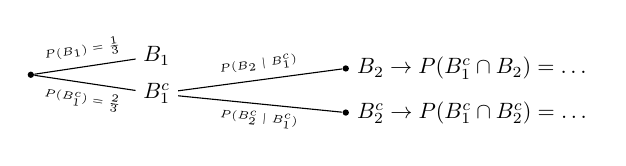
\begin{tikzpicture}[scale=0.8, every node/.style={transform shape}]
        \node[fill, circle, minimum size=1mm, inner sep=0] (O) at (0,1) {};
        \node[] (B1) at (2,1.3) {$B_1$};
        \node[] (B1c) at (2, 0.7) {$B_1^c$};
        \node[label=right:{$B_2 \rightarrow P(B_1^c \cap B_2) = \dots$}, fill, circle, minimum size=1mm, inner sep=0] (B2) at (5, 1.1) {};
        \node[label=right:{$B_2^c \rightarrow P(B_1^c \cap B_2^c) = \dots$}, fill, circle, minimum size=1mm, inner sep=0] (B2c) at (5, 0.4) {};
        \draw (O)  -- node[above, sloped] {\tiny{$P(B_1) = \frac{1}{3}$}} (B1);
        \draw (O) -- node[below, sloped] {\tiny{$P(B_1^c) = \frac{2}{3}$}} (B1c);
        \draw (B1c) -- node[above, sloped] {\tiny{$P(B_2\mid B_1^c)$}} (B2);
        \draw (B1c) -- node[below, sloped] {\tiny{$P(B_2^c\mid B_1^c)$}} (B2c);
    \end{tikzpicture}

\subsection{bayes' theorem}
Suppose a sample space $S$ is a union of mutually disjoint events $B_1, B_2, \dots, B_n$ and $A$ is an event in $S$.
\\* For $k \in \mathbb{Z}$ and $1 \leq k \leq n$, 
\begin{center}
    $P(B_k\mid A) = \frac{P(A \mid B_k) \cdot P(B_k)}{\sum\limits^n_{i=1}\big(P(A \mid B_i) \cdot P(B_i)\big)}$
\end{center}

\subsection{independent events}
\begin{center}
    $A$ and $B$ are \textbf{independent} \textit{iff}
    \\* $P(A \cap B) = P(A) \cdot P(B)$

    \hfill \break
    $A$, $B$ and $C$ are \textbf{pairwise independent} \textit{iff}
    \\* 1. $P(A \cap B) = P(A) \cdot P(B)$
    \\* 2. $P(B \cap C) = P(B) \cdot P(C)$
    \\* 3. $P(A \cap C) = P(A) \cdot P(C)$
    
    \hfill \break
    $A$, $B$ and $C$ are \textbf{mutually independent} \textit{iff}
    \\* 1. $A$, $B$ and $C$ are pairwise independent
    \\* 2. $P(A \cap B \cap C) = P(A) \cdot P(B) \cdot P(C)$

\end{center}
\end{multicols}

\pagebreak

\begin{center}
    \begin{tabular}{>{\color{black}}r | c | c}
        \multicolumn{3}{>{\color{black}}c}{LOGICAL EQUIVALENCES} 
        \\ \hline 
        commutative laws 
            & $p \land q \equiv q \land p$
            & $p \lor q \equiv q \lor p$
        \\ associative laws
            & $(p \land q) \land r \equiv p \land (q \land r)$
            & $(p \lor q) \lor r \equiv p \lor (q \lor r)$
        \\ distributive laws
            & $p \land (q \lor r) \equiv (p \land q) \lor (p \land r)$
            & $p \lor (q \land r) \equiv (p \lor q) \land (p \lor r)$
        \\ identity laws
            & $p \land true \equiv p$
            & $p \lor false \equiv p$
        \\ idempotent laws
            & $p \land p \equiv p$
            & $p \lor p \equiv p$
        \\ universal bound laws
            & $p \lor true \equiv true$
            & $p \land false \equiv false$
        \\ negation laws
            & $p \lor \lnot p \equiv true$
            & $p \land \lnot p \equiv false$
        \\ double negation law
            & $\lnot (\lnot p) \equiv p$
            & —
        \\ absorption laws
            & $p \lor (p \land q) \equiv p$
            & $p \land (p \lor q) \equiv p$
        \\ De Morgan's Laws
            & $\lnot (p \lor q) \equiv \lnot p \land \lnot q $
            & $\lnot (p \land q) \equiv \lnot p \lor \lnot q$
     \end{tabular}
     \quad
     \begin{tabular}{>{\color{black}}r | c | c}
        \multicolumn{3}{>{\color{black}}c}{SET IDENTITIES} 
        \\ \hline 
        commutative laws 
            & $A \cap B = B \cap A$
            & $A \cup B = B \cup A$
        \\ associative laws
            & $(A \cap B) \cap C = A \cap (B \cap C)$
            & $(A \cup B) \cup C = A \cup (B \cup C)$
        \\ distributive laws
            & $A \cap (B \cup C) = (A \cap B) \cup (A \cap C)$
            & $A \cup (B \cap C) = (A \cup B) \cap (A \cup C)$
        \\ identity laws
            & $A \cap U = A$
            & $A \cup \emptyset = A$
        \\ idempotent laws
            & $A \cap A = A$
            & $A \cup A = A$
        \\ universal bound laws
            & $A \cap \emptyset = \emptyset$
            & $A \cup U = U$
        \\ complement laws
            & $A \cap \overline{A} = \emptyset$
            & $A \cup \overline{A} = U$
        \\ double \bf{complement} law
            & $\overline{(\overline{A})} = A$
            & ---
        \\ absorption laws
            & $A \cup (A \cap B) = A$
            & $A \cap (A \cup B) = A$
        \\ De Morgan's Laws
            & $\overline{A \cup B} = \overline{A} \cap \overline{B}$
            & $\overline{A \cap B} = \overline{A} \cup \overline{B}$
     \end{tabular}
\end{center}
\begin{center}
    % \hrulefill \\
    \dotfill
\end{center}
\begin{multicols*}{3}
    \section{proven:}
    \begin{itemize}
        \item L1E1 - the product of 2 consecutive odd numbers is always odd.
        \item L1E5 - the difference between 2 consecutive squares is always odd
        \item L4E4 - the sum of any 2 even integers is even
        \item L4T4.6.1 - there is no greatest integer
        \item L4T4.3.1 - for all positive integers $a$ and $b$, if $a \vert b$, then $a \leq b$.
        \item L1P4.6.4 - for all integers $n$, if $n^2$ is even then $n$ is even
        \item L4T4.2.1 - all integers are rational numbers
        \item L4T4.2.2 - the sum of any 2 rational numbers is rational
        \item L1E7 - there exist irrational numbers $p$ and $q$ such that $p^q$ is rational
        \item L4T4.7.1 - $\sqrt{2}$ is irrational.
        \item L4T4.3.2 - the only divisors of $1$ are $1$ and $-1$.
        \item L4T4.3.3 - \bf{transitivity of divisibility} 
        \begin{itemize}
            \item if $a\vert b$ and $b \vert c$, then $a \vert c$.
        \end{itemize}
        \item L3T3.2.1 - \bf{negation of a universal statement}: 
        \begin{itemize}
            \item $\lnot (\forall x \in D, P(x)) \equiv \exists x \in D \mid \lnot P(x)$
        \end{itemize}
        \item L3T3.2.2 - \bf{negation of an existential statement}: 
        \begin{itemize}
            \item $\lnot (\exists x \in D \mid P(x)) \equiv \forall x \in D, \lnot P(x)$
        \end{itemize}
        \item L5T5.1.14 - there exists a unique set with no element. It is denoted by $\emptyset$.
        \item L5E5.3.7 - for all $A, B$: $(A \cap B) \cup (A \backslash B) = A$
        \item L5T5.3.11(1) - let $A, B$ be disjoint finite sets. Then $\vert A \cup B \vert = \vert A \vert + \vert B \vert$
        \item L5T5.3.11(2) - let $A_1, A_2, \dots, A_n$ be pairwise disjoint finite sets. Then $\vert A_1 \cup A_2 \cup \dots \cup A_n \vert = \vert A_1 \vert + \vert A_2 \vert + \dots + \vert A_n \vert$
        \item L5T5.3.12 - \bf{Inclusion-Exclusion Principle}: 
        \begin{itemize}
            \item for all finite sets $A$ and $B$, $\vert A \cup B \vert = \vert A \vert + \vert B \vert - \vert A \cap B \vert$
        \end{itemize} 
        \item L6T6.1.26 - \bf{associativity of function composition}: 
        \begin{itemize}
            \item $f\circ (g \circ h) = (f \circ g) \circ h$
        \end{itemize}
        \item L6P2.6.16 - \bf{uniqueness of inverses}: 
        \begin{itemize}
            \item If $g, g'$ are inverses of $f: A \to B$, then $g = g'$.
        \end{itemize} 
        \item E6.1.24 - $f \circ \text{id}_\text{A} = f$ and $\text{id}_\text{A} \circ f = f$
        \item T6.2.18 - bijective $\Iff$ has an inverse
        \item L7.3.19 - If $x \in \text{WFF}^+(\Sigma)$, then assigning false to all elements of $\Sigma$ makes $x$ evaluate to false.
        \item T7.3.20 - $\lnot( \forall x \in \text{WFF}(\Sigma), \exists y \in \text{WFF}^+(\Sigma) \ \ y \equiv x ) \equiv$
            $\exists x \in \text{WFF}(\Sigma) \ \ \forall y \in \text{WFF}^+(\Sigma) \ \ y \not\equiv x$
            aka $\lnot$ (not) must be included in the definition of WFF.
        \item L8.1.5 - Let $d, n \in \mathbb{Z}$ with $d \neq 0$. Then $d \mid n \Iff n/d \in \mathbb{Z}$ 
        \item L8.1.9 - Let $d, n \in \mathbb{Z}$. If $d \mid n$, then $-d \mid n$ and $d \mid -n$ and $-d \mid -n$ 
        \item L8.1.10 - Let $d, n \in \mathbb{Z}$. If $d \mid n$ and $d \neq 0$, then $\vert d \vert \leq \vert n \vert$ 
        \item L8.2.5 - \bf{Prime Divisor Lemma} (non-standard name):
        \begin{itemize}
            \item Let $n \in \mathbb{Z}_{\geq 2}$. Then $n$ has a prime divisor.
        \end{itemize}
        \item P8.2.6 - \bf{sizes of prime divisors}: 
        \begin{itemize}
            \item Let $n$ be a composite positive integer. Then $n$ has a prime divisor $p \leq \sqrt{n}$.
        \end{itemize}
        \item T8.2.8 - there are infinitely many prime numbers
        \item T8.3.13 - $\forall n \in \mathbb{Z}^+, \exists ! \ell \in \mathbb{Z}_{\geq 0}$ and $a_0, a_1, \dots, a_\ell \in \{0, 1, \dots, b - 1\}$ 
        such that <the definition of base-b representation> holds.
        \item L8.4.11 - If $x, y, r \in \mathbb{Z}$ such that $x \ mod \ y = r$, then $gcd(x, y) = gcd(y, r)$.
        \item Let $a, b, c, d \in \mathbb{Z}$ and $n \in \mathbb{Z}^+$ s.t. $a \equiv b \ (\Mod{n})$ and $c \equiv d \ (\Mod{n})$. 
        \begin{itemize}
            \item P8.6.6 - \bf{addition: } Then $a + c \equiv b + d \ (\Mod n)$
            \item P8.6.13 - \bf{multiplication: } Then $ac \equiv bd \ (\Mod n)$
        \end{itemize}
        \item T9.3.4 - Let $R$ be an equivalence relation on a set $A$. Then $A / R$ is a partition of A.
        \item T9.3.5 - If $\mathscr{C}$ is a partition of $A$, then there is an equivalence relation of $R$ on $A$ such that $A/R = \mathscr{C}$.
        \item L9.5.5 - Consider a partial order $\preccurlyeq$ on set $A$. 
        \begin{itemize}
            \item A smallest element is minimal.
            \item There is at most one smallest element.
        \end{itemize}
    \end{itemize}

    \subsection{abbreviations}
    \begin{itemize}
        \item L - lemma
        \item E - example
        \item P - proposition
        \item T - theorem
    \end{itemize}
\end{multicols*}

\end{document}